%
% 		Funciones comunes a todos los módulos.
%
%
\section{Entorno de OpenErp - Funciones Comunes}
\begin{figure}[h]
 \centering
 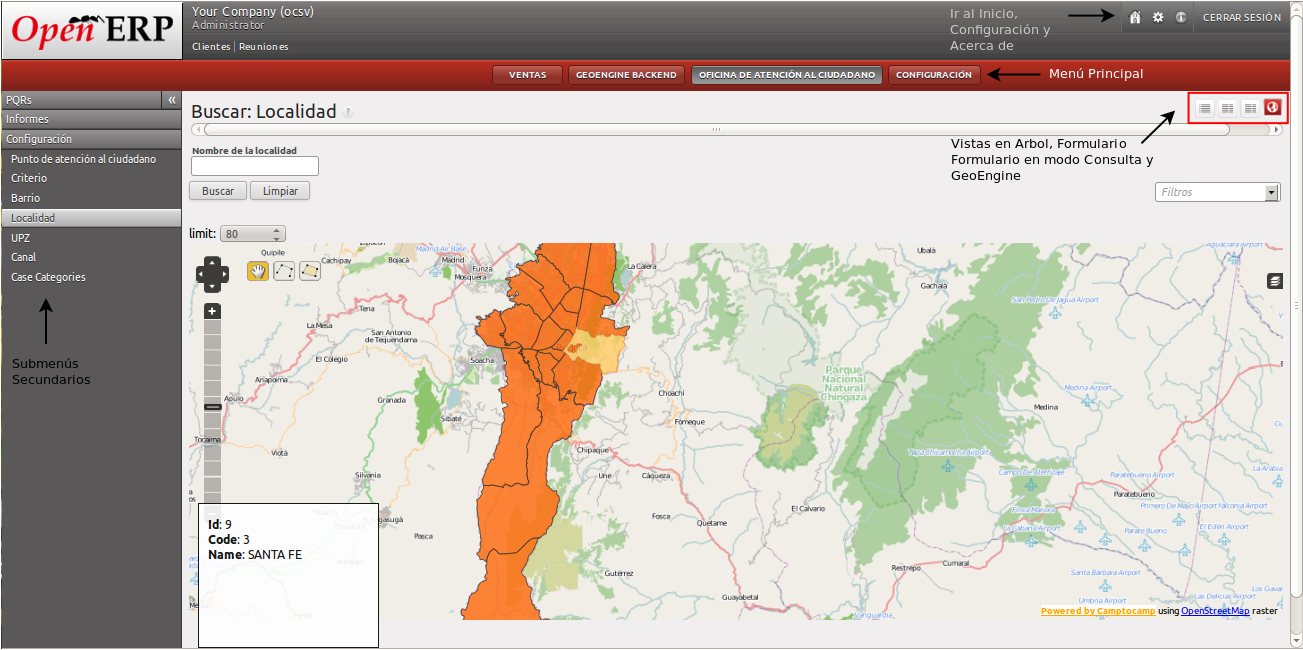
\includegraphics[width=17cm,height=8cm]{./Imagenes/enviroment.png}
 % Login.png: 1289x610 pixel, 96dpi, 34.10x16.14 cm, bb=0 0 967 457
 \caption{Panorama General de OpenErp}
 \label{fig:enviroment}
\end{figure}

\begin{figure}
 \centering
 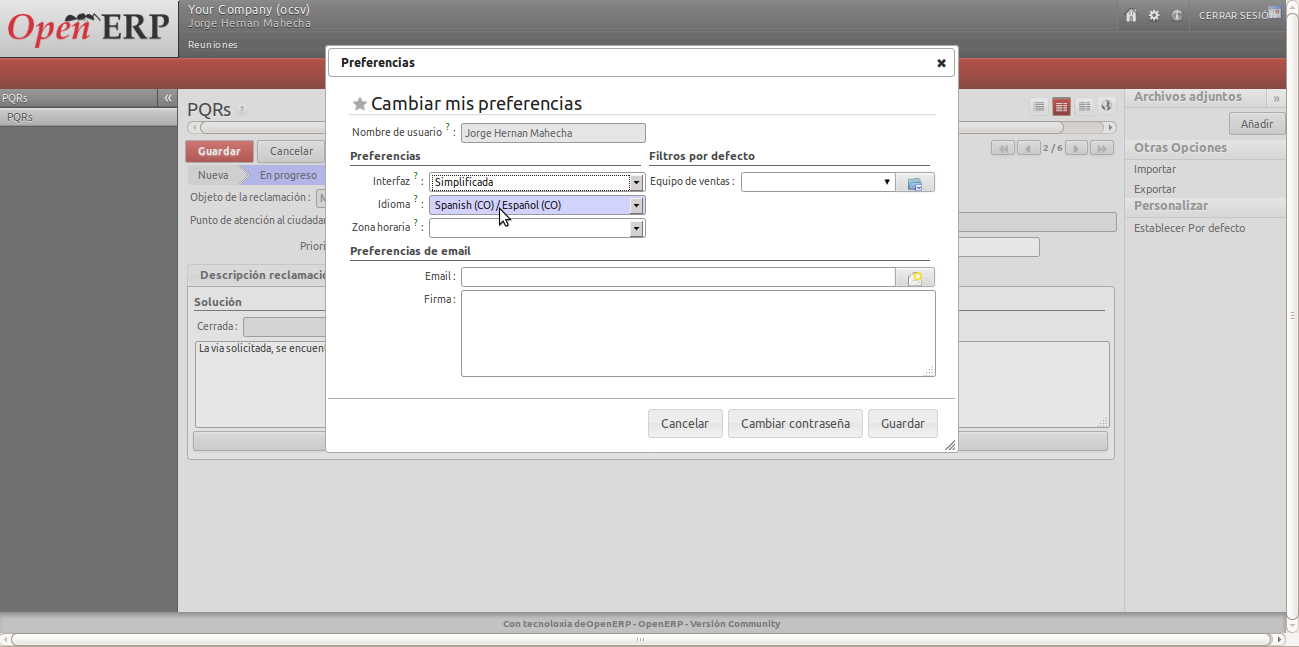
\includegraphics[width=17cm,height=8cm]{./Imagenes/configuracion.png}
 % Login.png: 1289x610 pixel, 96dpi, 34.10x16.14 cm, bb=0 0 967 457
 \caption{Ventana de configuración de preferencias y cambio de contraseña}
 \label{fig:configuracion}
\end{figure}

\subsection {Cambiar contraseña y cambiar configuración de Idioma}
\begin{itemize}
 \item Hacer clic en el botón \textbf{Configuración}, que tiene forma de rueda dentada y se encuentra en la 
 superior derecha, a la izquierda del botón \textbf{Cerrar Cesión} (Ver figura \ref{fig:enviroment}).
 \item Se desplega una ventana emergente con las opciones de configuración (figura \ref{fig:configuracion}).
 \item En la parte inferior se encuentra el botón  \textbf{Cambiar Contraseña}.
 \item En la parte media de la ventana se encuentran los idiomas disponibles para la aplicación, por defecto
 se encuentra el Inglés y el Idioma Local (Spanish-CO). 
\end{itemize}


\subsection{Tipos de Vistas}
Existen en OpenErp varios tipos de vistas:
\begin{itemize}
 \item Lista (Arbol). 
 \item Formulario.
 \item Geoengine. (Geográfica).
 \item Kanban.
 \item Gant.
 \item Calendario.
 \item Gráfico (Grafico de Barras). 
\end{itemize}
Las vistas disponibles para una aplicación se encuentran en la parte superior derecha, debajo de la barra del menú principal
(Ver figura \ref{fig:enviroment}). Para pasar de una vista a otra simplemente se hace clic en el icono correspondiente.
\subsection{Iconos Comúnes}

\begin{enumerate}
 \item \textbf{Barra de Estados} 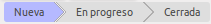
\includegraphics[width=4cm,height=0.5cm]{./Imagenes/barraestados.png}:
  Muchos de los objetos que conforman OpenErp cambian de estado de acuerdo de acuerdo a como se desarrolla el
  flujo de trabajo. La barra de estado muestra como va cada proceso que se está llevando a cabo, su ubicación es variable
  y generalmente el estado actual de un proceso está demarcado con un color diferente.
 \item \textbf {Icono de entidades relacionadas} 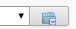
\includegraphics[width=2cm,height=0.5cm]{./Imagenes/entidadesrelacionadas.png}: Cuando un campo tiene este icono al lado,
 significa que se está relacionando otra tabla dentro de la aplicación, por ejemplo cuando se menciona una empresa o un contacto, se está mostrando la información una tabla
 de empresas o una tabla de de contactos. El ícono significa además que se puede  \textbf{crear}, \textbf{editar} o \textbf{buscar} el campo deseado. 
 Sin embargo estas opciones estarán disponibles para el usuario de acuerdo con su perfil, los permisos están clasificados para leer, modificar, crear
 o eliminar un registro dentro de una tabla específica. 
 
\end{enumerate}




